%\normalsize
In the era of the Higgs discovery and scrupulous searches
for signals of new physics at the LHC it is crucial
to have accurate Standard Model (SM) predictions for
many hard scattering processes such as the Higgs production at the LHC.
A most common approach to calculate the SM cross sections for  
such reactions is to use perturbative QCD collinear factorisation:
%is with perturbative QCD using a (collinear) factorisation approach: 
%{\small
\begin{equation}
\small
\begin{array}{l}
\sigma^{pp\rightarrow H + X}(\alpha_s,\mu_r,\mu_f) = \\[1mm] 
\sum\limits_{a,b}\,  \int\limits_{0}\limits^{1} dx_1 \int\limits_{0}\limits^{1} dx_2\, f_a(x_1,\alpha_s,\mu_F) 
 f_b(x_2,\alpha_s,\mu_F) 
\times \, \hat{\sigma}^{ab \rightarrow H + X}(x_1,x_2;\alpha_s,\mu_R,\mu_F).\\[3mm]
\end{array}
%\sigma^{pp\rightarrow H + X}(\alpha_s,\mu_r,\mu_f) = 
%\sum_{a,b} \int_{0}^{1} dx_1 \int_{0}^{1} dx_2 f_a(x_1) 
% f_b(x_1,\alpha_s,\mu_F) \times \hat{\sigma}^{ab \rightarrow H + X}(x_1,x_2;\alpha_s,\mu_R,\mu_F)
\label{eq:fact}
\end{equation}
%}
Here the cross section $\sigma^{pp\rightarrow H + X}$ for inclusive
Higgs production is expressed
as a convolution of Parton Distribution Functions (PDF) $f_a$ and $f_b$
with the partonic cross section
% that describe
%the 
$\hat{\sigma}^{ab \rightarrow H + X}$.
%
The PDFs describe 
the probability of finding a specific parton $a$ ($b$) in the first (second) proton
carrying the fraction $x_1$ ($x_2$) of its momentum.
%
The sum in Eq.~\ref{eq:fact} over $a$ and $b$ is over all different kind of partons,
i.e. gluons and the various quarks and antiquarks flavours, that are considered
as the constituents of the proton.
%
Both the PDFs and the partonic cross section depend on the strong coupling
constant $\alpha_s$ and the factorisation and renormalisation scales
$\mu_F$ and $\mu_R$.
%
The partonic cross sections are calculable in pQCD while
the PDFs cannot be determined solely with pQCD but are assumed 
to be universal (that is process independent).
%
This make it possible to use different scattering reactions 
to constrain the PDFs; in particular one can use specific reaction data 
for determining the PDFs and then take these PDFs for
predicting other processes via Eq.~\ref{eq:fact}.
%

Key information on the PDFs is provided by the Deep Inelastic Scattering (DIS) data 
from the $ep$ collider HERA.
%
For instance, the gluon density relevant
for calculating the dominant gluon gluon fusion contribution to Higgs production
at the LHC can be accurately determined from the HERA data alone.
%
%Despite being often plagued by larger perturbative uncertainties,
Specific data from the Tevatron $p\bar{p}$ and the LHC $pp$ collider
can help to further constrain the PDFs.
%
The most sensitive processes are
Drell Yan production, W and Z asymmetries, top quark production, jet production
and  others.
%

\fitter is a QCD analysis tool based on QCD factorisation that aims at 
determining precise PDFs by integrating/using all the PDF sensitive information
from HERA, Tevatron and the LHC.
%
The processes that are currently included in \fitter framework are listed in Tab.~\ref{tab:proc}.
%
\begin{table}
\begin{tabular}{|l|l|l|l|}
\hline
Process &  Diagram & Theory      & Available \\
Process &          & calculation &  data\\
\hline
DIS NC   & & & HERA \\
DIS CC   & & & HERA \\
DIS jets & & & HERA\\
DIS heavy quark prod & & & HERA \\
\hline
$pp(\bar p)$ Drell Yan & & Applgrid & Tevatron, LHC \\
                       & & Sapronov  &  \\
$pp(\bar p)$ W charge asym & & Applgrid & Tevatron, LHC \\
$pp(\bar p)$ top & & & Tevatron, LHC \\
$pp(\bar p)$ jets & & Applgrid & Tevatron, LHC \\
                  & & FastNLO  &  \\
$pp(\bar p)$ DY+heavy quark & & Applgrid & LHC \\
\hline
\end{tabular}
\caption{The list of processes available in \fitter.}
\label{tab:proc}
\end{table}
%

The basic functionality of HERAFitter is shown in Fig.~\ref{fig:flow} and consists
of four parts: {\bf needs to update figure!}
\begin{figure}[!ht]
   \centering
   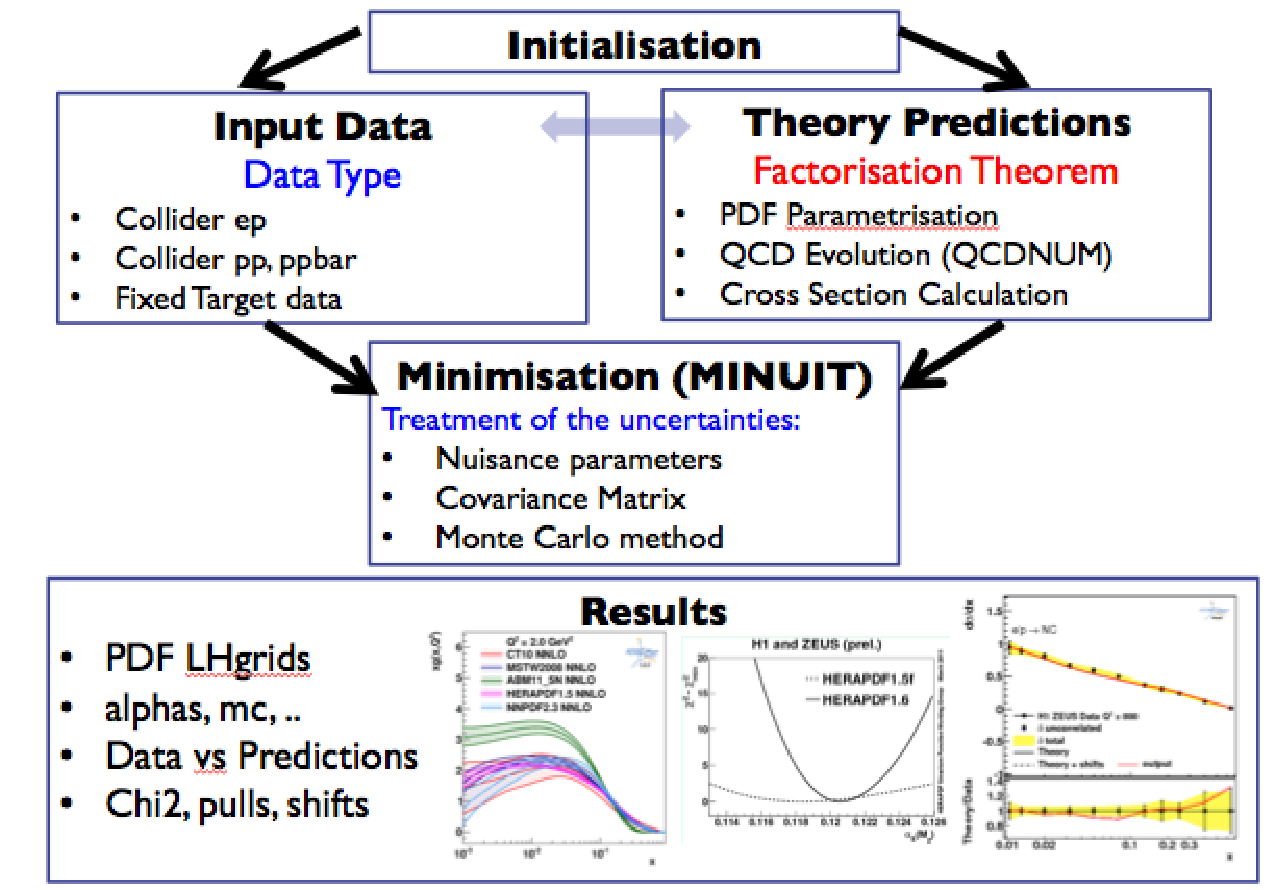
\includegraphics[width=8cm]{flow.pdf}
   \caption{Schematic structure of the \fitter program.} 
 \label{fig:flow}
\end{figure}
\begin{itemize}
\item 
Input data: All relevant cross section data from the various reactions
are stored internally in \fitter with the full information on their uncorrelated and correlated
uncertainties.
\item
    Theory: Predictions are obtained using the factorisation approach (Eq.~\ref{eq:fact}).
The PDFs are parametrised at a starting scale $Q_0$  by a certain functional form.
They depend on a set of fit parameters $\vec{p}$. 
The PDFs are  evolved from $Q_0$ to the factorisation scale $\mu_F$ using 
Dokshitzer-Gribov-Lipatov-Altarelli-Parisi 
(DGLAP)~\cite{Gribov:1972ri,Gribov:1972rt,Lipatov:1974qm,
Dokshitzer:1977sg,Altarelli:1977zs} evolution equations 
as implemented in QCDNUM~\cite{qcdnum} 
and then multiplied (Eq.~\ref{eq:fact}) with the hard parton cross sections calculated by
a specific theory program (also listed in Tab.~\ref{tab:proc}).
\item
Minimization: A least square fit is performed, constructing a 
$\chi^2$ from the input data and the theory prediction.
The $\chi^2$ is  minimized iteratively 
with respect to the PDF parameters using the MINUIT program.
%
%Fitted values of $\vec{p}$ and estimated uncertainties are obtained.
%The fitted parameters $\vec(p)$ and obtained from the uncertainties of the parameters are determined (from chi2+1???)
%
\item
Output: The fitted parameters $\vec{p}$ and their estimated covariances
from MINUIT are provided.
The resulting PDFs are provided in a ready to be used LHAPDF library form
and can be graphically 
discplayed at arbitrary scales with their one sigma uncertainties bands.
To demonstrate the fit consistency, plots are provided 
in which the input data are compared to the fitted theory predictions.
\end{itemize}
%
%This paper provides a comprehensive description of  \\
%the \fitter\ package.
%which is designed for analysis of the High Energy Physics data.
%The package has been developed by members of the H1 and ZEUS collaborations
%with an exclusive support of different theoretical groups.
%The main purpose of the \fitter\ package is analysis of the 
%data from the $e^{\pm}p$, $p\bar{p}$, and $pp$ collider experiments
%information obtained from the deep inelastic scattering experiments
%and the determination of the parton density functions (PDFs).
%The broad range of data taken from the $e^{\pm}p$, $p\bar{p}$, and $pp$ collider experiments can be
%studied by the package. 

The outline of this paper is as follows.
%
Section~\ref{sec:theory} discusses the various processes 
and corresponding theoretical calculations 
that are available in \fitter.
%
Section~\ref{sec:method} elucidates the 
methodology of determining PDF based on various approaches {\bf (what do you mean here
by approaches?)} and $\chi^2$ definitions used in the
minimisation.
%
Specific applications of the package are given in
section ~\ref{sec:examples}. 
%
{\bf add something more here?.}
